\documentclass[openright,10pt,onecolumn]{report}

% % % Packages
\usepackage{afterpage}
\usepackage{sectsty}
% citation
\usepackage[noadjust]{cite}
% header and footer
\usepackage[english]{babel}
\usepackage[utf8]{inputenc}
\usepackage{fancyhdr}
\usepackage[table,xcdraw]{xcolor}
\usepackage{url}
\usepackage{multicol}

\usepackage[hyperfootnotes=false]{hyperref}
%cross reference
\usepackage{hyperref}
\hypersetup{
    colorlinks=true,
    linkcolor=black,
    hyperfootnotes = false,
    filecolor=magenta,      
    urlcolor=cyan,
    pdftitle={Sharelatex Example},
    bookmarks=true,
    pdfpagemode=FullScreen,
    citecolor=black
}

%caption
\usepackage{caption} 
\captionsetup[table]{skip=2pt}

% Margin configuration

%geometry of main textbook
\usepackage[left=2cm, right=2cm, top=3cm , bottom=3cm , headsep=.75cm , voffset =.55cm]{geometry}

\usepackage{algorithm}
\usepackage{pseudocode}
\renewcommand\headrulewidth{1.5pt}

% Header and footer configuration
\pagestyle{fancy}

\renewcommand{\chaptername}{}
\renewcommand{\chaptermark}[1]{%
\markboth{#1}{}}
\renewcommand{\sectionmark}[1]{\markright{\thesubsection\ #1}}

\fancyhf{}
\fancyhead[RO]{\begin{picture}(0,0) \put(-75,0){\includegraphics[width=3.4cm]{Team_Logo}} \end{picture}}
\lhead{\large\nouppercase{\leftmark}}
\cfoot{\thepage}

\usepackage[pdftex]{graphicx}
\usepackage{subcaption}
\usepackage{indentfirst}
\usepackage{tikz}
\usepackage{tabularx,booktabs}
\newcolumntype{C}{>{\centering\arraybackslash}X} % centered version of "X" type
\setlength{\extrarowheight}{1pt}
\usepackage{lipsum}
\usetikzlibrary{shapes,arrows}
\usepackage[export]{adjustbox}

\usepackage{mwe}
\usepackage{float}
\usepackage{amssymb}
\usepackage{arydshln}
\usepackage{amsmath}
\usepackage{booktabs,siunitx,multirow,enumitem,tabularx}
\usepackage{pifont}% http://ctan.org/pkg/pifont
\newcommand{\chmark}{\ding{51}}%
\newcommand{\xmark}{\ding{55}}%
\usepackage{tasks}
\usepackage{exsheets}
\usepackage{color,soul}
\usepackage{wrapfig, blindtext}
\usepackage{pdfpages}
\usepackage{xparse} 

% Acronyms
\usepackage{acronym}

% Set line spacing
\usepackage{setspace}

% Configuration for title
\usepackage{titlesec}
%%%\newcommand{\bigrule}{\titlerule[0.5mm]}
%%%\renewcommand{\rmdefault}{bch} 
\titleformat{\chapter}[display]
{\normalfont}{}
{0pt}{\LARGE\bfseries}                      %left/raght %up/down 
\titlespacing*{\chapter} {0pt}{-30pt}{5pt}
\titlespacing*{\section} {0pt}{-3pt}{3pt}
\titlespacing*{\subsection} {0pt}{-1pt}{3pt}
\titlespacing*{\subsubsection} {0pt}{-1pt}{3pt}


%header and footer in chapter page
\usepackage{etoolbox}
\makeatletter
\let\ps@plain\ps@fancy
\makeatother
%Reference name
\makeatletter
\def\thebibliography#1{\chapter*{References\@mkboth
  {REFERENCES}{REFERENCES}}\list
  {[\arabic{enumi}]}{\settowidth\labelwidth{[#1]}\leftmargin\labelwidth
\advance\leftmargin\labelsep
\usecounter{enumi}}
\def\newblock{\hskip .81em plus .93em minus .07em}
\sloppy\clubpenalty4000\widowpenalty4000
\sfcode`\.=1000\relax}
\makeatother

\renewcommand{\listfigurename}{List of Figures}
\renewcommand{\listtablename}{List of Tables}

\setcounter{tocdepth}{1}

\begin{document}
\LARGE
%%%%% First page

\thispagestyle{empty}
\begin{centering}

  {\color{white}AIAA 2018-2019 Undergraduate Space System Design Competition}
  \begin{center}
    {\color{white}\line(1,0){470}} 
   \end{center}
   
  {\color{white}Submitted by}\\
 
  {\color{white}Sharif University Team: ShadX New Horizon}
  \begin{center}
    {\color{white}\line(1,0){470}} 
   \end{center}
     
  \begin{figure}[hbtp]   
    \centering
    {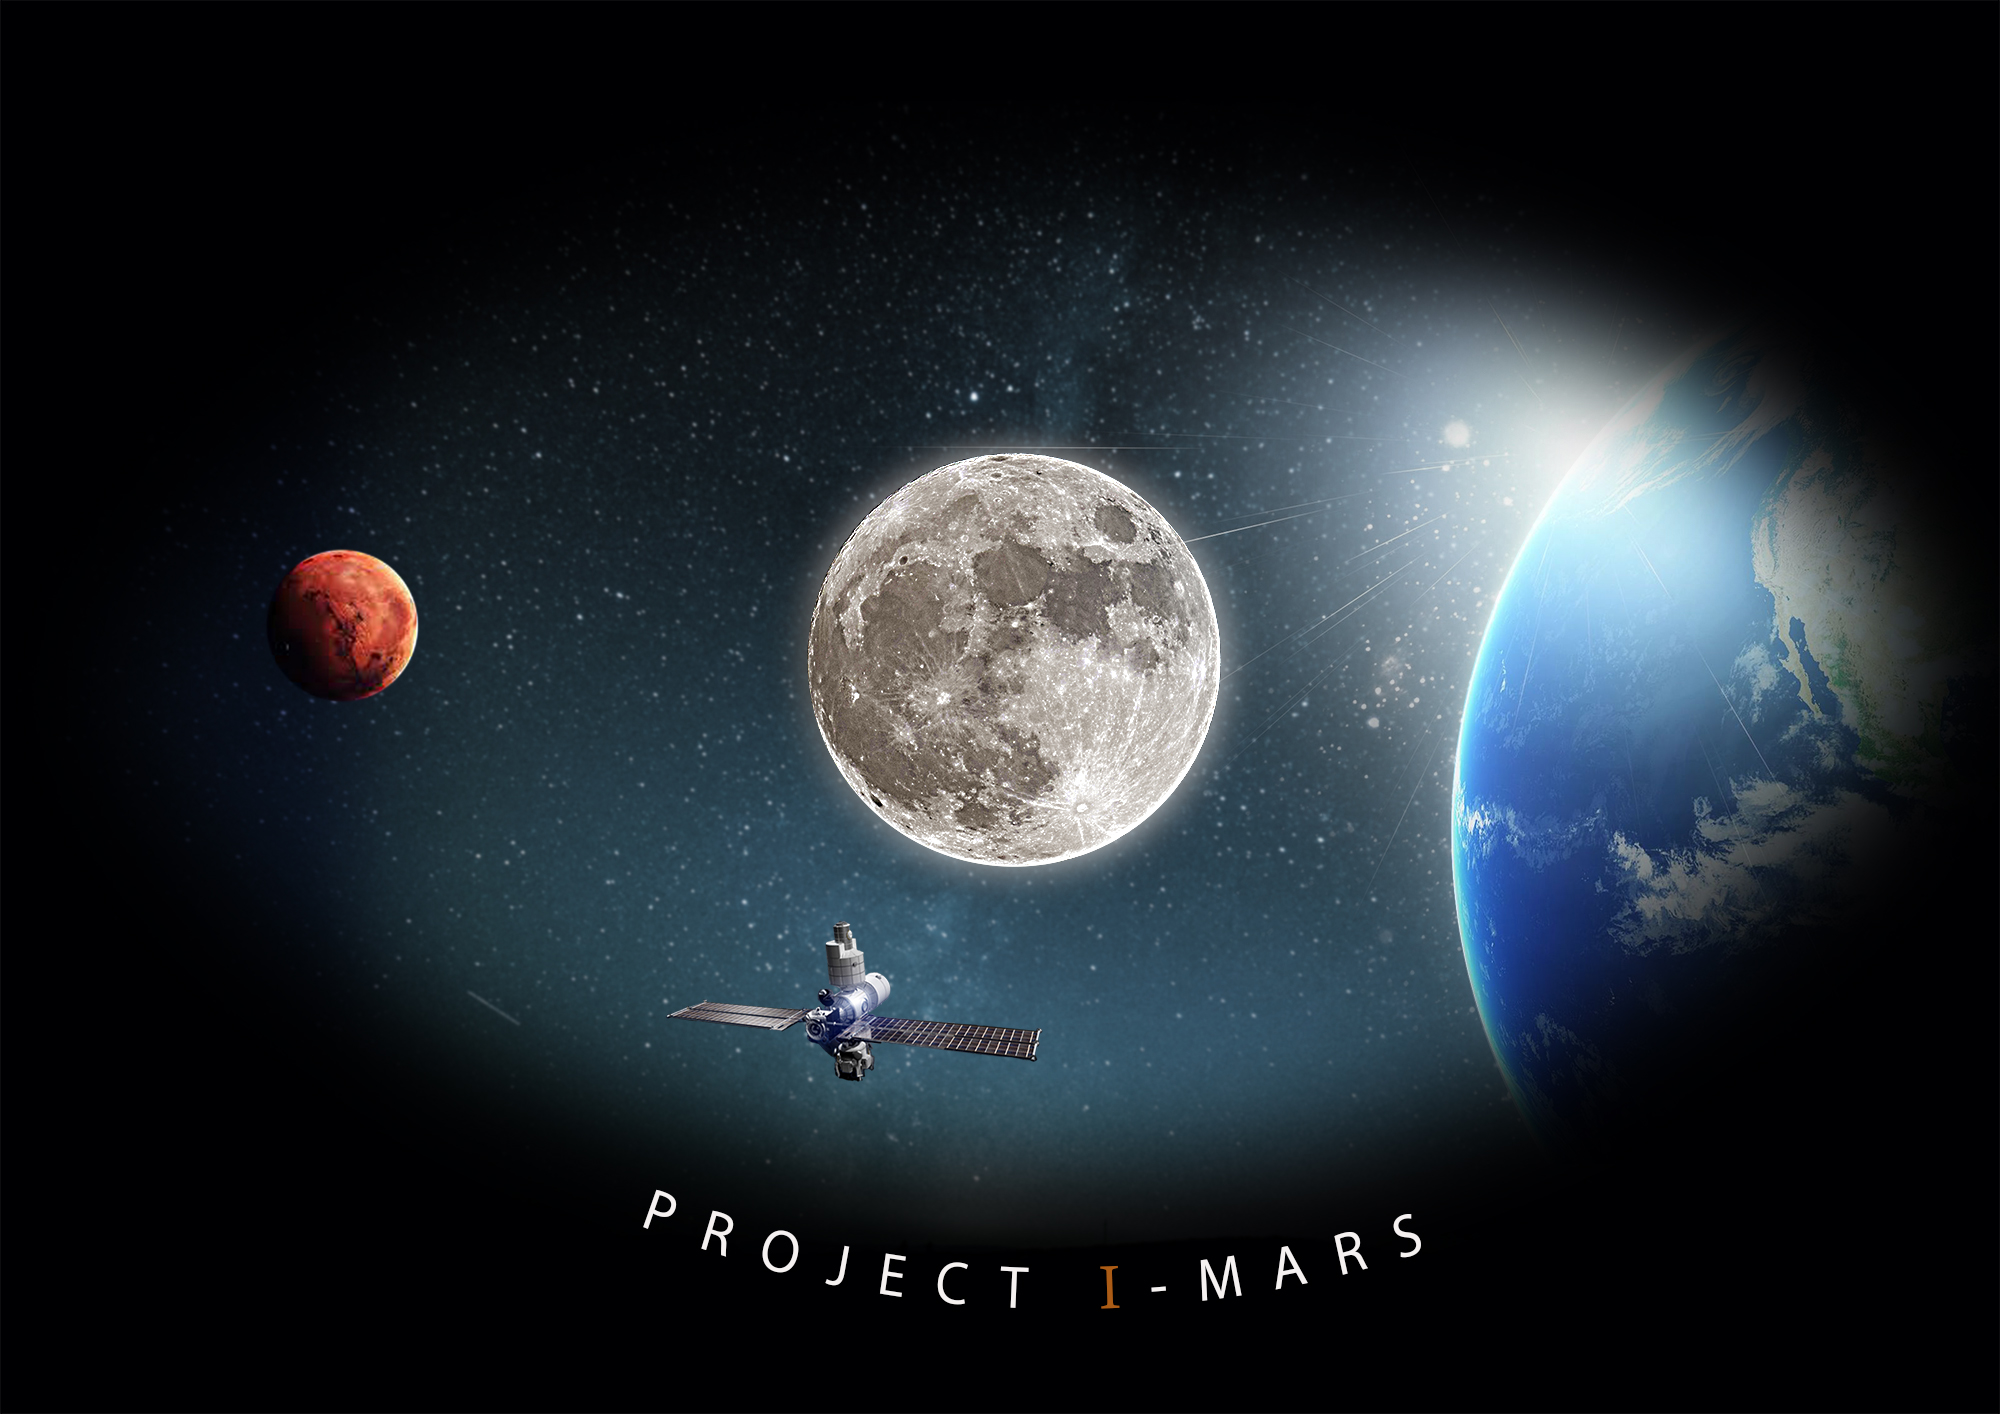
\includegraphics[width=\linewidth]{First_page}}
  \end{figure}
  \pagecolor{black}\afterpage{\nopagecolor}
  
  
  {\color{white}\textbf{Intelligent Multi surface Access Reusable Spacecraft}}\\
  
  {\color{white}\today}  

\end{centering}

%% Acknowledgments


\normalsize
\newpage%avoid page numbering in first page
%Contents
\pagenumbering{roman}

\newpage
\singlespacing

\renewcommand{\contentsname}{Table of Contents}

\begin{multicols}{2}
  \tableofcontents
\end{multicols}

\begin{multicols}{2}
\listoffigures
\end{multicols}

\addcontentsline{toc}{chapter}{List of Figures}
\begin{multicols}{2}
\listoftables
\end{multicols}

\addcontentsline{toc}{chapter}{List of Tables}
\afterpage{%
\newgeometry{left=2cm, right=2cm, top=2.7cm , bottom=2.7cm , headsep=1.25cm , voffset =1.25cm}

\twocolumn
\let\oldleftmark=\leftmark
\chapter*{Acronyms}
\renewcommand{\leftmark}{Acronyms}
\addcontentsline{toc}{chapter}{Acronyms}
\begin{acronym}

\end{acronym}

\newenvironment{absolutelynopagebreak}
  {\par\nobreak\vfil\penalty0\vfilneg
   \vtop\bgroup}
  {\par\xdef\tpd{\the\prevdepth}\egroup
   \prevdepth=\tpd}

\begin{absolutelynopagebreak}
\onecolumn

\chapter*{Acknowledgments}
\doublespacing

\end{absolutelynopagebreak}
\onecolumn
\clearpage

\newpage

\pagenumbering{arabic}
\let\leftmark=\oldleftmark
\restoregeometry
}
\include{chapters/history/history}
\afterpage{%
\newgeometry{left=2cm, right=2cm, top=2.7cm , bottom=2.7cm , headsep=.75cm , voffset =.55cm}
\include{chapters/requirements_definition/mission_definition}
\clearpage
\restoregeometry
}
\afterpage{%
\newgeometry{left=2cm, right=2cm, top=2.7cm , bottom=2.7cm , headsep=.75cm , voffset =.55cm}
\include{chapters/executive_summary/executive_summary}
\clearpage
\restoregeometry
}
\afterpage{%
\newgeometry{left=2cm, right=2cm, top=2.7cm , bottom=2.7cm , headsep=.75cm , voffset =.55cm}
\include{chapters/fact_sheet/fact_sheet}
\clearpage
\restoregeometry
}
\afterpage{%
\newgeometry{left=2cm, right=2cm, top=2.7cm , bottom=2.7cm , headsep=.75cm , voffset =.55cm}
\include{chapters/mission_overview/mission_overview1}
\clearpage
\restoregeometry
}
\afterpage{%
\newgeometry{left=2cm, right=2cm, top=2.7cm , bottom=2.7cm , headsep=.75cm , voffset =.55cm}
\include{chapters/science/science2}
\clearpage
\restoregeometry
}
\afterpage{%
\newgeometry{left=2cm, right=2cm, top=2.7cm , bottom=2.7cm , headsep=.75cm , voffset =.55cm}
\include{chapters/configuration/configuration1}
\clearpage
\restoregeometry
}
\afterpage{%
\newgeometry{left=2cm, right=2cm, top=2.7cm , bottom=2.7cm , headsep=.75cm , voffset =.55cm}
\include{chapters/trajectory/trajectory6} 
\clearpage
\restoregeometry
}
\afterpage{%
\newgeometry{left=2cm, right=2cm, top=2.7cm , bottom=2.7cm , headsep=.75cm , voffset =.55cm}
\include{chapters/propulsion/propulsion6} 
\clearpage
\restoregeometry
}
\afterpage{%
\newgeometry{left=2cm, right=2cm, top=2.7cm , bottom=2.7cm , headsep=.75cm , voffset =.55cm}
\include{chapters/control/control11}
\clearpage
\restoregeometry
}
\afterpage{%
\newgeometry{left=2cm, right=2cm, top=2.7cm , bottom=2.7cm , headsep=.75cm , voffset =.55cm}
\include{chapters/life_support/life_support1}
\clearpage
\restoregeometry
}
\afterpage{%
\newgeometry{left=2cm, right=2cm, top=2.7cm , bottom=2.7cm , headsep=.75cm , voffset =.55cm}
\include{chapters/thermal/thermal5}
\clearpage
\restoregeometry
}
\afterpage{%
\newgeometry{left=2cm, right=2cm, top=2.7cm , bottom=2.7cm , headsep=.75cm , voffset =.55cm}
\include{chapters/power/power6}
\clearpage
\restoregeometry
}
\afterpage{%
\newgeometry{left=2cm, right=2cm, top=2.7cm , bottom=2.7cm , headsep=.75cm , voffset =.55cm}
\include{chapters/structure/structure}
\clearpage
\restoregeometry
}
\afterpage{%
\newgeometry{left=2cm, right=2cm, top=2.7cm , bottom=2.7cm , headsep=.75cm , voffset =.55cm}
\include{chapters/communication/communication1}
\clearpage
\restoregeometry
}
\afterpage{%
\newgeometry{left=2cm, right=2cm, top=2.7cm , bottom=2.7cm , headsep=.75cm , voffset =.55cm}
\include{chapters/cost/cost6}
\clearpage
\restoregeometry
}
\afterpage{%
\newgeometry{left=2cm, right=2cm, top=2.7cm , bottom=2.7cm , headsep=.75cm , voffset =.55cm}
\include{chapters/risk_assesment/risk_assesment3}
\clearpage
\restoregeometry
}
\afterpage{%
\newgeometry{left=2cm, right=2cm, top=2.7cm , bottom=2.7cm , headsep=.45cm , voffset =.25cm}
\include{chapters/schedule/schedule}
\clearpage
\restoregeometry
}
\afterpage{%
\newgeometry{left=2cm, right=2cm, top=2.7cm , bottom=2.7cm , headsep=.45cm , voffset =.25cm}
\include{chapters/summary_table/summary_table}
\clearpage
\restoregeometry
}

\singlespacing


\bibliography{%file address}

\bibliographystyle{IEEEtran}

\addcontentsline{toc}{chapter}{References}
\end{document}



